\documentclass[xcolor=pdftex,dvipsnames,table]{beamer}

\usepackage{graphicx}

%\usepackage{beamerthemesplit}
%\usetheme{CambridgeUS}
\usetheme{Warsaw}
\usecolortheme{seahorse}
%\setbeamertemplate{theorems}[numbered]

% Abbreviations
\newcommand{\bbC}{\mathbb{C}}
\newcommand{\bbD}{\mathbb{D}}
\newcommand{\bbH}{\mathbb{H}}
\newcommand{\bbN}{\mathbb{N}}
\newcommand{\bbR}{\mathbb{R}}
\newcommand{\bbZ}{\mathbb{Z}}
\newcommand{\calF}{\mathcal{F}}
\newcommand{\gve}{\varepsilon}
\newcommand{\gvp}{\varphi}
\newcommand{\ga}{\alpha}
\newcommand{\gb}{\beta}
\newcommand{\gd}{\delta}
\newcommand{\gl}{\lambda}
\newcommand{\go}{\omega}
\newcommand{\gr}{\gamma}
\newcommand{\gs}{\sigma}
\newcommand{\gt}{\theta}
\newcommand{\gz}{\zeta}
\newcommand{\gD}{\Delta}
\newcommand{\gG}{\Gamma}
\newcommand{\gO}{\Omega}
\newcommand{\gR}{\Gamma}
\newcommand{\half}{\frac{1}{2}}
\renewcommand{\Re}{\text{Re}\,}
\renewcommand{\Im}{\text{Im}\,}
\newcommand{\area}{\text{area}\,}
\newcommand{\rad}{\text{rad}\,}
\newcommand{\crad}{\text{crad}\,}
\newcommand{\diam}{\text{diam}\,}
\newcommand{\dist}{\text{dist\,}}
\newcommand{\lcap}{\text{cap}}
\newcommand{\dcap}{\text{dcap}}
\newcommand{\hcap}{\text{hcap}}
\newcommand{\capD}{\text{cap}_{\mathbb{D}}}
\newcommand{\capH}{\text{cap}_{\mathbb{H}}}
\newcommand{\Caratheodory}{Carath\'{e}odory}
\newcommand{\Holder}{H\"{o}lder}

% Environments
\theoremstyle{definition}
\newtheorem*{conjecture}{Conjecture}
\newtheorem{question}{Question}
\newtheorem{answer}{Answer}
\newtheorem{exercise}{Exercise}
\newtheorem{remark}{Remark}

\title{Half-plane Capacity and Conformal Radius\\
       (joint work with Steffen Rohde)}
\author{Carto Wong}
\institute{University of Washington}
\date{December 12, 2011\\The Chinese University of Hong Kong}

\begin{document}

\maketitle

\section{Motivation}

\begin{frame}
  Let $\gR$ be a slit in the unit disk $\bbD$ going from $a \in \partial \bbD$ to 0.
  \begin{question}
    What is a ``canonical'' parametrization of $\gR$?
  \end{question}
  \begin{figure}
    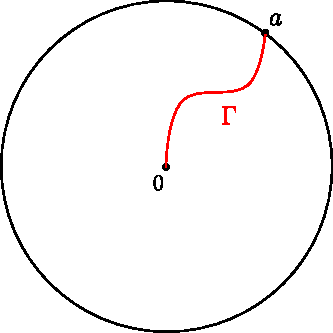
\includegraphics[scale=0.8]{radialSlit.pdf}
  \end{figure}
\end{frame}

\begin{frame}
  \frametitle{Two cases}
  \begin{figure}
    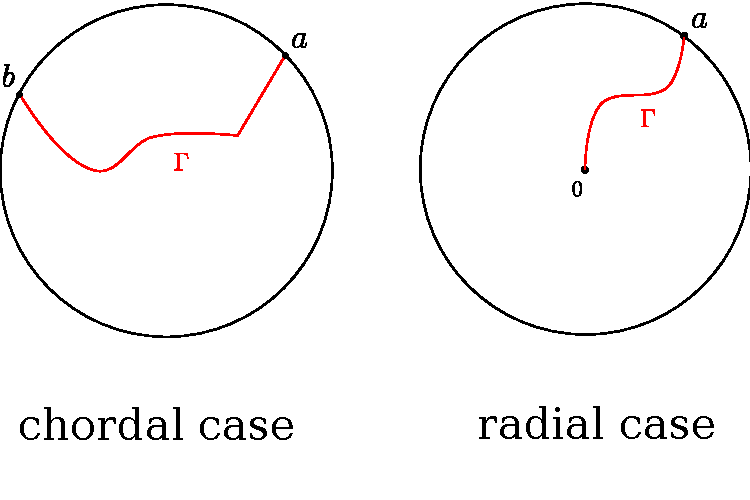
\includegraphics[scale=0.6]{twoCases.pdf}
  \end{figure}
\end{frame}

\begin{frame}
  \frametitle{Radial case}
  Suppose $\gr \colon (0,T) \to \bbD$ is a slit. There is a unique conformal mapping
  \[
    f_t \colon \bbD \to \bbD \setminus \gr([0,t])
  \]
  satisfying $f_t(0) = 0$ and $f_t'(0) > 0$. \onslide<2->{We define the {\color{Red!100} ``disk capacity''}
  \[
      \dcap(\gR_t) := - \log f_t'(0).
  \]}
  \vspace{-0.8in}  
  \begin{figure}
    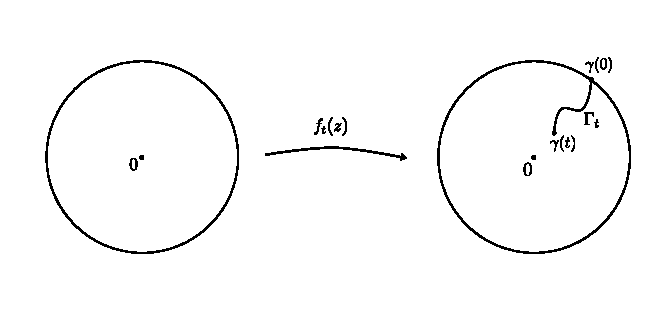
\includegraphics{radial_f(z,t).pdf}
  \end{figure}
\end{frame}

\begin{frame}
  \begin{question}
    What is a ``canonical'' parametrization of $\gR$?
  \end{question}
  \begin{figure}
    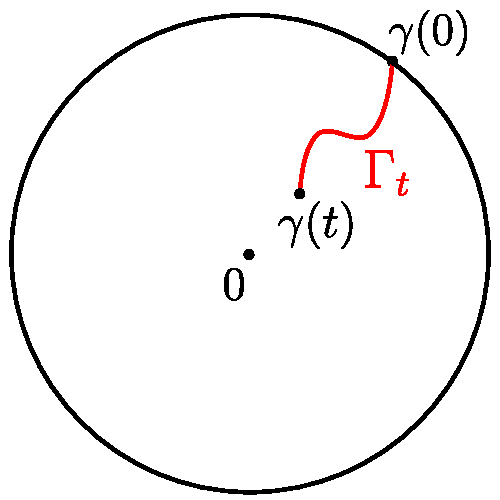
\includegraphics[scale=0.3]{radialSlit_02.pdf}
  \end{figure}
  \begin{answer}
    Parametrize the slit so that $\dcap(\gR_t) = t$.
  \end{answer}
  \vspace{0.1in}
  Used in radial Schramn-Loewner Evolution (SLE)
\end{frame}

\begin{frame}
  \frametitle{Reason}
  \begin{theorem}
    Suppose the slit is parametrized so that {\color{Red!100} $\dcap(\gR_t) = t$}. Then the conformal
    mapping $f_t(z)$ satisfies the (radial) Loewner differential equation
    {\color{black!30}
      \[
          \partial_t f_t(z) = - f_t'(z) \, \frac{\gl(t) + z}{\gl(t) - z}
      \]
      for some continuous function $\gl(t)$ with $\left|\gl(t)\right| \equiv 1$.
    }
  \end{theorem}
  \vspace{-0.4in}
  \begin{figure}
    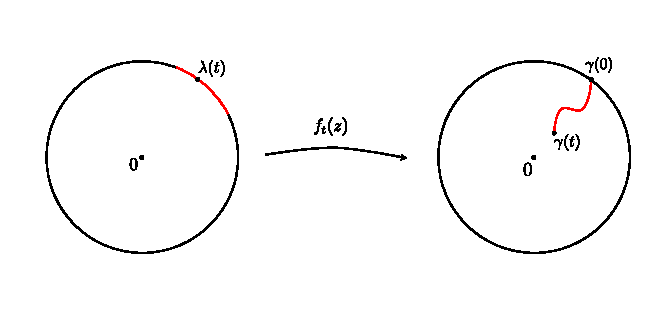
\includegraphics[scale=0.9]{radial_f(z,t)_02.pdf}
  \end{figure}
\end{frame}

\begin{frame}
  \frametitle{Chordal (half-plane) case}
  Hydrodynamic normalization:
  \[
      g_t(z) = z + \frac{a_1(t)}{z} + \frac{a_2(t)}{z^2} + \cdots
      \qquad (z \to \infty)
  \]
  \onslide<2->{The {\color{Red!100} half-plane capacity} of $\gR_t$ is defined as
  \[
      \hcap(\gR_t) := \lim_{z \to \infty}
      z \left[ g_t(z) - z \right] \geq 0.
  \]}
  \vspace{-0.3in}
  \begin{figure}
    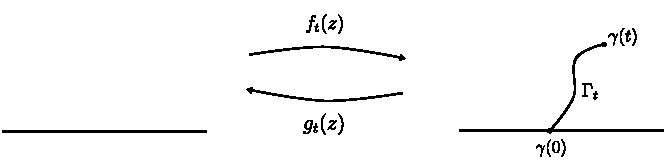
\includegraphics[scale=0.6]{chordal_f(z,t).pdf}
  \end{figure}
  \onslide<3->{
  \begin{example}
    $A = [0,i]$, $g(z) = \sqrt{z^2 + 1} = z + \frac{1}{2z} + \cdots$ and $\hcap(A) = \half$.
  \end{example}}
\end{frame}

\begin{frame}
  \begin{question}
    What is a ``canonical'' parametrization of $\gR$?
  \end{question}
  \begin{figure}
    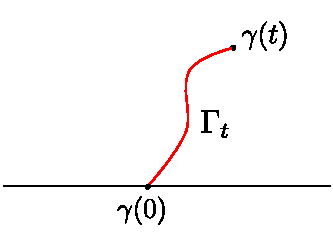
\includegraphics[scale=0.5]{chordalSlit_02.pdf}
  \end{figure}
  \begin{answer}
    Parametrize the slit so that $\hcap(\gR_t) = 2t$.
  \end{answer}
  \vspace{0.1in}
  Used in chordal Schramm-Loewner Evolution (SLE)
\end{frame}

\begin{frame}
  \frametitle{Chordal Loewner differential equation}
  \begin{theorem}
    Suppose the slit is parametrized so that {\color{Red!100} $\hcap(\gR_t) = 2t$}. Then $g_t(z)$
    satisfies the (chordal) Loewner differential equation
    {\color{black!30}
    \[
        \partial_t g_t(z) = \frac{2}{g_t(z) - \gl(t)}
    \]
    for some continuous real-valued function $\gl(t)$.}
  \end{theorem}
  \begin{figure}
    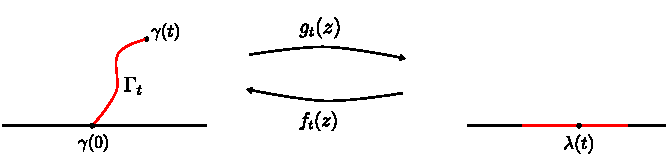
\includegraphics[scale=0.9]{chordal_f(z,t)_02.pdf}
  \end{figure}
\end{frame}

\begin{frame}
  \frametitle{Basic properties of $\hcap(A)$}
  \begin{itemize}
    \setlength{\itemsep}{0.3in}
    \item  monotone: \[A \subseteq B \Rightarrow \hcap(A) \leq \hcap(B).\]
    \item  invariant under horizontal translation: for any $x \in \bbR$, \[\hcap(A + x) = \hcap(A).\]
    \item  scaling property: for any $r > 0$, \[\hcap(r A) = r^2 \hcap(A).\]
  \end{itemize}
\end{frame}

\section{Main result}

\begin{frame}
  \begin{question}
    Find a geometric quantity that is comparable to $\hcap(A)$.
  \end{question}
  
  \vspace{0.2in}
  
  Scaling property: $\hcap(r A) = r^2 \hcap(A)$. Some candidates are
  \vspace{0.1in}
  \begin{itemize}
    \item  $\area(A)$
    \item  $\diam(A)^2$
    \item  $\text{height}(A)^2$
    \item  $\diam(A) \times \text{height}(A)$
  \end{itemize}
  \vspace{0.1in}
  \onslide<2->{They all fail!}
\end{frame}

\begin{frame}
  \frametitle{Counter-example}
  $\hcap(A)$ and $\diam(A)^2$ are not comparable:
  \[
      \hcap([0,e^{i \ga \pi}]) = \frac{1}{2} \ga^{1-2\ga} (1-\ga)^{2 \ga - 1} \to 0
  \]
  as $\ga \to 0$.
  \begin{figure}
    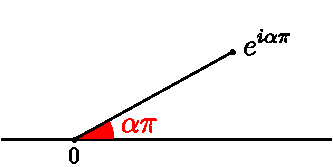
\includegraphics[scale=0.9]{ray.pdf}
  \end{figure}
\end{frame}

\begin{frame}
  \frametitle{Notation}
  For $z \in \bbH$, define
  \[
    \begin{aligned}
      \onslide<1->{T(z) &= \text{triangular region in the figure below}} \\
      \onslide<2->{T(A) &= \bigcup_{z \in A} T(z)} 
    \end{aligned}
  \]
  \begin{figure}
    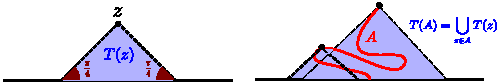
\includegraphics[scale=1.3]{T(A).pdf}
  \end{figure}
\end{frame}

\begin{frame}
  \frametitle{Main result}
  \begin{theorem}
    There are constants $c_1$,~$c_2 > 0$ such that
    \[
        c_1 \cdot \area(T(A)) \leq \hcap(A) \leq c_2 \cdot \area(T(A))
    \]
    for all $A$.
  \end{theorem}
  \vspace{-0.2in}
  \begin{figure}
    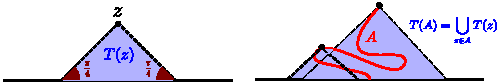
\includegraphics[scale=1.3]{T(A).pdf}
  \end{figure}
\end{frame}

\begin{frame}
  \frametitle{S(A)}
  Whitney squares: 
  \[
      \begin{aligned}
          S_{n,k} &= [k 2^n, (k+1) 2^n] \times [2^n, 2^{n+1}] \qquad (n, k \in \bbZ)\\
          S(A) &= \bigcup_{j} S_j
      \end{aligned}
  \]
  \begin{figure}
    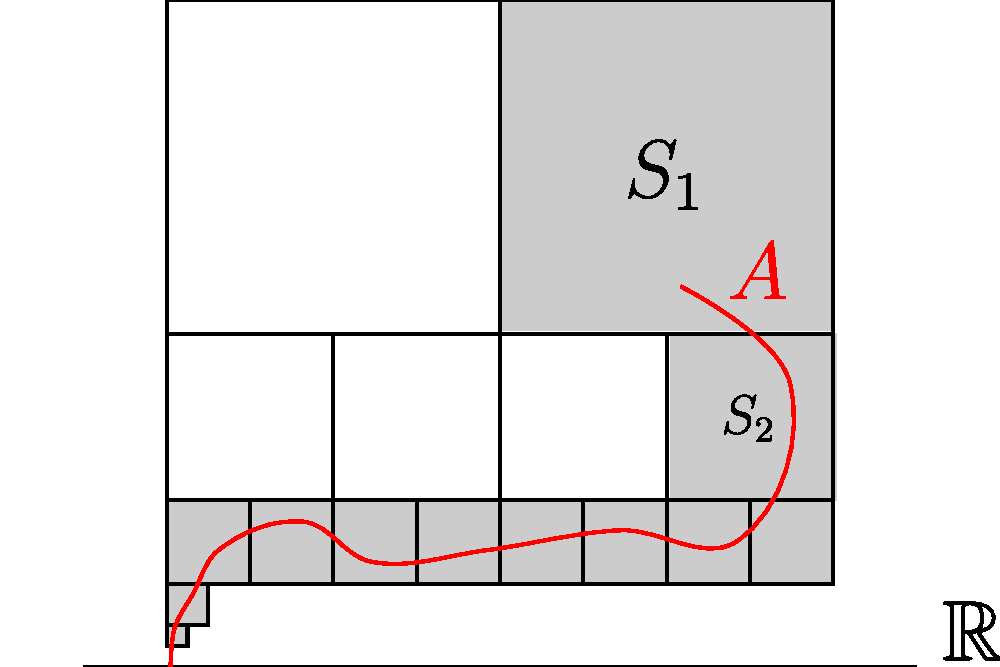
\includegraphics[scale=0.4]{S(A).pdf}
  \end{figure}
\end{frame}


\begin{frame}
  \frametitle{Comparable quantities}
  With absolute constants,
  \[
    \area N(A) \asymp \area S(A) \asymp \area T(A).
  \]
  \begin{figure}
    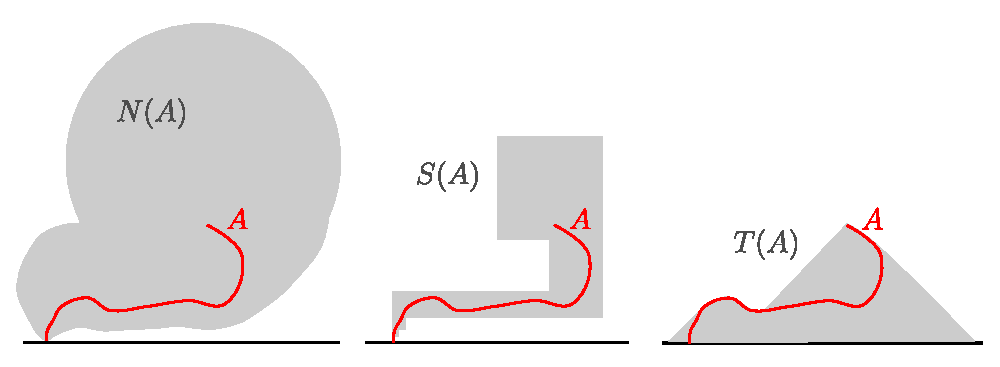
\includegraphics[scale=0.6]{geomQuantity.pdf}
  \end{figure}
\end{frame}

\begin{frame}
  \frametitle{History of the problem}
  \begin{enumerate} \setlength{\itemsep}{.2in}
    \item[2001]  Steffen Rohde and Michel Zinsmeister: showed a similar result
                 for conformal radius when $A$ is ``already fat''.\\
                 \vspace{.1in}
                 \onslide<2->{Wong: proof using the probabilistic definition of
                 $\hcap(A)$. (2008 manuscript, to be part of a thesis.)
                 The result became ``folklore''.}
    \item[2009]  \onslide<3->{Steven Lalley, Gregory Lawler, Hariharan Narayanan: proved
                 the ``ball version''. The proof also uses probabilistic argument.}
    \item[2010]  \onslide<4->{(with Steffen Rohde) a non-probabilistic proof, using a
                           known result about conformal radius.}                        
  \end{enumerate}
\end{frame}

\section{Sketch of proof}

\begin{frame}
  \frametitle{Outline of a proof for the main result}
  3 ingredients in our proof: \vspace{.2in}
  \begin{enumerate} \setlength{\itemsep}{.2in}
    \item  an equivalent problem about dcap (conformal radius)
    \item  a ``fattening lemma''
    \item  a lemma for the fat case (``Variation of conformal radius''
              Steffen Rohde and Michel Zinsmeister, 2001)
  \end{enumerate}
\end{frame}

\begin{frame}
  \frametitle{Half-plane capacity and conformal radius}
  $\dcap(B) = - \log f'(0) \asymp 1 - f'(0)$ for $B \subseteq \{ \half \leq \left| z \right| < 1 \}$.
  \begin{lemma}
    \[
      \lim_{y \to \infty} \frac{\dcap(B_y)}{\hcap(y^{-1}A)} = 2.
    \]  
  \end{lemma}
  \begin{figure}
      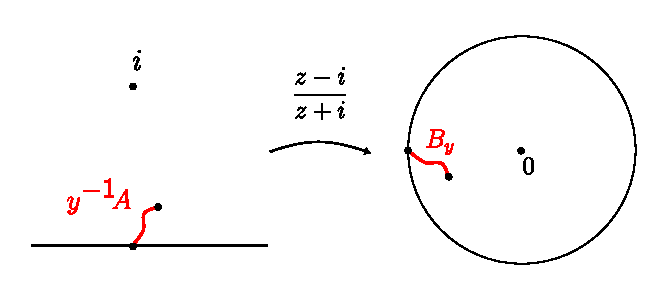
\includegraphics[scale=0.6]{hcap_dcap.pdf}
  \end{figure}
  \vspace{-0.1in}
\end{frame}

\begin{frame}
  \frametitle{Equivalent problems}
  \begin{problem}
    \[
        \hcap(A) \asymp \area N(A)
    \]
    for any slit $A \subseteq \bbH$.
  \end{problem}
  \vspace{.2in} is equivalent to \vspace{.2in}
  \begin{problem}
    \[
        \dcap(B) \asymp \area N(B)
    \]
    for any slit $B \subseteq \left\{ \half \leq \left|z\right| < 1 \right\}$.
  \end{problem}    
\end{frame}

\begin{frame}
  \frametitle{Outline of a proof for the main result}
  3 ingredients in our proof: \vspace{.2in}
  \begin{enumerate} \setlength{\itemsep}{.2in}
    \item  {\color{black!30} an equivalent problem about dcap (conformal radius)}
    \item  a ``fattening lemma''
    \item  a lemma for the fat case (``Variation of conformal radius''
              Steffen Rohde and Michel Zinsmeister, 2001)
  \end{enumerate}
\end{frame}

\begin{frame}
  \frametitle{Fattening lemma}
  \begin{figure}
    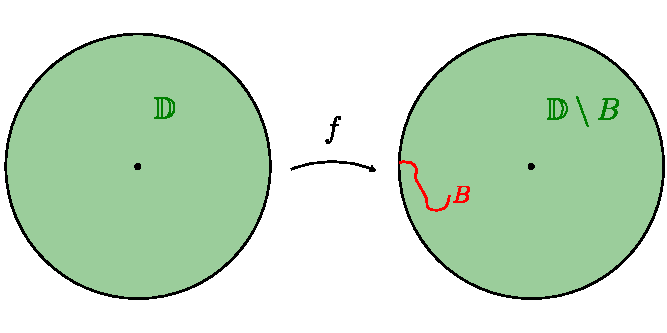
\includegraphics[scale=0.8]{fattening_03.pdf}
  \end{figure}
  \[
      \dcap(B) = - \log \left| f'(0) \right| \asymp 1 - \left| f'(0) \right|
  \]  
\end{frame}

\begin{frame}
  \frametitle{Fattening lemma}
  \begin{figure}
    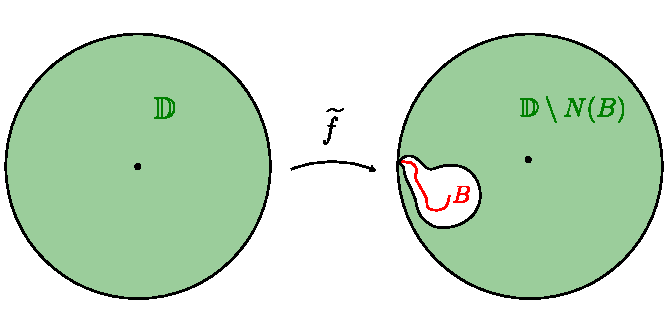
\includegraphics[scale=0.8]{fattening_04.pdf}
  \end{figure}
  \[
      \dcap \, N(B) = - \log \left| \widetilde{f}'(0) \right| \asymp 1 - \left| \widetilde{f}'(0) \right|
  \]  
\end{frame}

\begin{frame}
  \frametitle{Fattening lemma}
  \begin{lemma}[Fattening lemma]
    For $B \subseteq \{ \frac{1}{2} \leq \left| z \right| < 1 \}$,
    \[
        {\color{black!30} \dcap(B) \leq} \dcap \, N(B) \leq c \, \dcap(B).
    \]  
  \end{lemma}
  \begin{figure}
    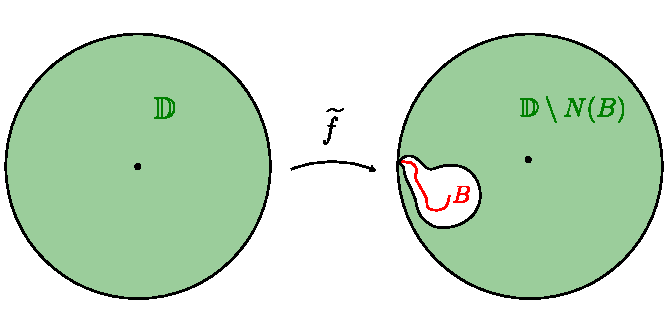
\includegraphics[scale=0.8]{fattening_04.pdf}
  \end{figure}
\end{frame}

\begin{frame}
  \frametitle{Lower bound for $\dcap(B)$}
  Let $f \colon \bbD \to \bbD \setminus B$ be conformal with $f(0) = 0$.
  \[
      \begin{aligned}
          f(z) &= a_1 z + a_2 z^2 + \cdots \\
          \area(\bbD \setminus B) &= \pi \left( \left|a_1\right|^2 + 2 \left|a_2\right|^2 + 3 \left|a_3\right|^2 + \cdots \right) \\
                                                      &\geq \pi \left| a_1\right|^2 \\
           \area(B) &\leq \pi (1 - \left|a_1\right|^2) \asymp 1 - \left| a_1 \right| \asymp \dcap(B)                                           
      \end{aligned}
  \]
  By the fattening lemma,
  \[
      \dcap (B) \gtrsim \dcap N(B) \gtrsim \area N(B).
  \]    
\end{frame}

\begin{frame}
  \frametitle{Proof of fattening lemma (sketch)}
  Decompose $\bbD$ into dyadic layers $D_n = \{ \frac{1}{2^{n+1}} < 1 - \left|z\right| \leq \frac{1}{2^n} \}$.
   \[
      \begin{aligned}
          \dcap(B) &= - \log \left| f'(0) \right| \\
          &= \frac{1}{2 \pi} \int_{\partial \bbD} - \log \left| f(\gz) \right| \, d\gz \\
          &\asymp \sum_{n=1}^{\infty} \frac{\go_n(0)}{2^n},
      \end{aligned}
  \]
  where $\go_n(z) = \go(z, B_n, \bbD \setminus B_n)$ and $B_n = B \cap D_n$.
\end{frame}

\begin{frame}
  \frametitle{Proof of fattening lemma (sketch)}
  Similarly,
   \[
       \dcap \, N(B) \asymp \sum_{n=1}^{\infty} \frac{\widetilde{\go}_n(0)}{2^n}.
  \]
  The fattening lemma follows if one can show that
  \[
      \widetilde{\go}_n(z) \lesssim \go_{n-1}(z) + \go_n(z) + \go_{n+1}(z)
  \]
  for $z \in \bbD \setminus N(B)$ and all $n$.
\end{frame}

\begin{frame}
  \frametitle{Harmonic measure estimate}
  It is in general not true that
  \[
      \widetilde{\go}_n(z) \lesssim \go_n(z)
  \]
  for $z \in \bbD \setminus N(B)$.
  \begin{figure}
      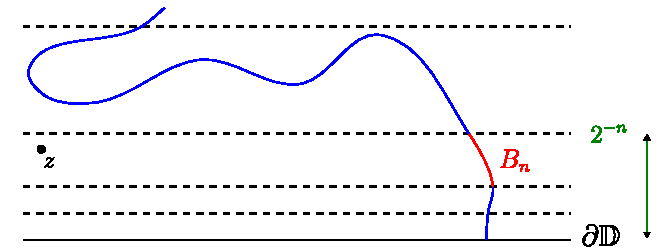
\includegraphics[scale=0.8]{harmEst.pdf}
  \end{figure}
\end{frame}

\begin{frame}
  \frametitle{Harmonic measure estimate}
  By taking 3 terms, we have
  \[
       \widetilde{\go}_n(z) \lesssim \go_{n-1}(z) + \go_n(z) + \go_{n+1}(z)
  \]
  for $z \in \bbD \setminus N(B)$.
  \begin{figure}
      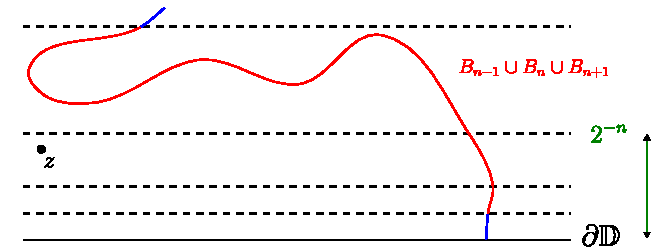
\includegraphics[scale=0.8]{harmEst_01.pdf}
  \end{figure}
\end{frame}
 
\begin{frame}
  \frametitle{Outline of a proof for the main result}
  3 ingredients in our proof: \vspace{.2in}
  \begin{enumerate} \setlength{\itemsep}{.2in}
    \item  {\color{black!30} an equivalent problem about dcap (conformal radius)
    \item  a ``fattening lemma''}
    \item  a lemma for the fat case (``Variation of conformal radius''
              Steffen Rohde and Michel Zinsmeister, 2001)
  \end{enumerate}
\end{frame}

\begin{frame}
  \frametitle{The fat case}
  \begin{lemma}[Rohde and Zinsmeister, 2001]
    If $B = \bigcup_{j=1}^n Q_j$ is a union of disjoint dyadic squares, then
    \[
        \dcap(B) \asymp \area(B).
    \]
  \end{lemma}
  \begin{figure}
    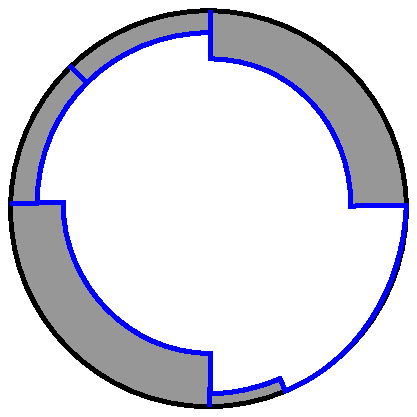
\includegraphics[scale=0.6]{fatCase.pdf}
  \end{figure}
\end{frame}

\begin{frame}
  \frametitle{Upper bound of \dcap(B)}
  Cover $B$ by dyadic squares in a minimal way. Call the larger set $Q(B) \supseteq B$.
  \begin{figure}
      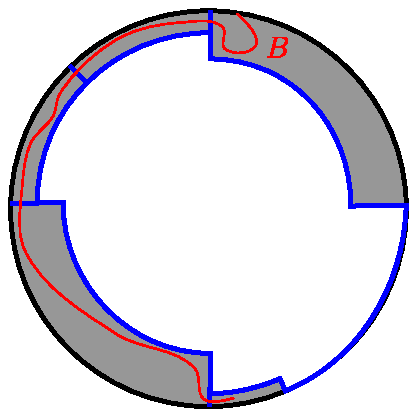
\includegraphics[scale=0.6]{Q(B).pdf}
  \end{figure}
  \[
      \dcap(B) \leq \dcap Q(B) \lesssim \area Q(B) \lesssim \area N(B).
  \]
\end{frame}

\begin{frame}
  \frametitle{The fat case}
  \begin{lemma}[Rohde and Zinsmeister, 2001]
    If $B = \bigcup_{j=1}^n Q_j$ is a union of disjoint dyadic squares, then
    \[
        \dcap(B) \asymp \area(B).
    \]
  \end{lemma}
  {\color{blue} Sketch of proof.} WLOG, $\area(Q_1) \leq \area(Q_2) \leq \dots \leq \area(Q_n)$.
  Using induction, it suffices to show that
  \[
      \dcap \left( \bigcup_{j=1}^{m} Q_j \right) - \dcap \left( \bigcup_{j=1}^{m-1} Q_j \right) \asymp
      \area(Q_m)
  \]
  for all $m$.
\end{frame}

\begin{frame}
  \frametitle{The induction step}
  \begin{figure}
    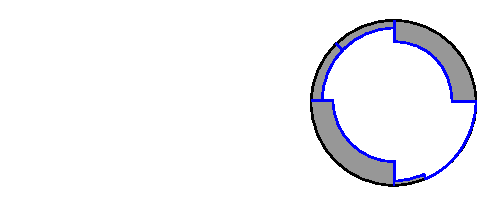
\includegraphics[scale=1]{removeOneSquare_01.pdf}
  \end{figure}
\end{frame}

\begin{frame}
  \frametitle{The induction step}
  \begin{figure}
    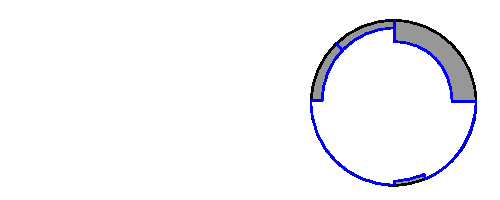
\includegraphics[scale=1]{removeOneSquare_02.pdf}
  \end{figure}
\end{frame}

\begin{frame}
  \frametitle{The induction step}
  \begin{figure}
    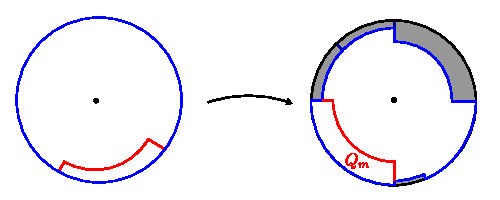
\includegraphics[scale=1]{removeOneSquare_03.pdf}
  \end{figure}
  On the right side,
  \[
      \go \asymp \diam(Q_m) \asymp \sqrt{\area(Q_m)}.
  \]
\end{frame}

\begin{frame}
  \frametitle{The induction step}
  \begin{figure}
    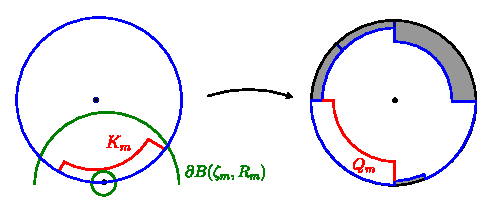
\includegraphics[scale=1]{removeOneSquare_04.pdf}
  \end{figure}
  On the left side, the red curve is bounded between two circles $\partial B(\gz_m, \rho R_m)$ and $\partial B(\gz_m, R_m)$
  with center $\gz_m \in \partial \bbD$, where {\color{blue} $\rho \in (0,1)$ is an absolute constant}. Moreoever,
  \[
      \go \asymp R_m \asymp \sqrt{\dcap(K_m)}.
  \]
\end{frame}

\begin{frame}
  \begin{center}
    \huge{Thank you!}
  \end{center}
  \vspace{.2in}
  These slides are available at\\
  {\color{blue} https://github.com/cartowong/halfplane-capacity}  
\end{frame}

\end{document}